\maincolumn{
\begin{center}
    %%%%%%%%%%%%%%%%%%%%%%%%%%
    %%%%%%%%% Header %%%%%%%%%
    %%%%%%%%%%%%%%%%%%%%%%%%%%
    ARFC: \textbf{Advanced Reactors} and \textbf{Fuel Cycles}\\
    \fontsizetitle
    PI: {\textbf{Prof. Katy Huff}}, \href{mailto:kdhuff@illinois.edu}{\underline{kdhuff}@\underline{illinois.edu}}
    \newline\vspace{-3em}
    \rule{\textwidth}{5pt}
    \newline\vspace{-1.5em}

    %%%%%%%%%%%%%%%%%%%%%%%%%
    %%%% Research Areas %%%%%
    %%%%%%%%%%%%%%%%%%%%%%%%%
    \textcolor{black}{
        \begin{minipage}{.32\linewidth}
            \begin{tcolorbox}[colback=white, colframe=black, width=\linewidth, height=1.55\linewidth, boxrule=1pt]
                \researcharea{Coupled Multiphysics of Advanced Reactors}
                \newline\vfill
                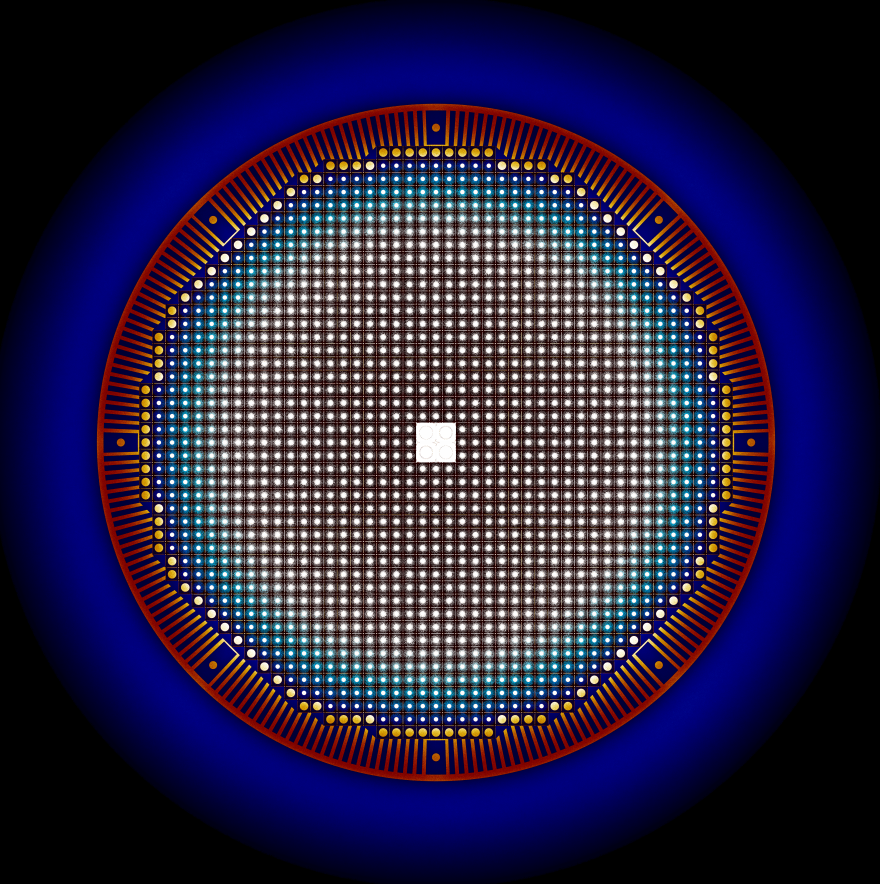
\includegraphics[width = \textwidth]{img/multiphysics.png}
                \vfill
            \end{tcolorbox}
        \end{minipage}
        \begin{minipage}{.32\linewidth}
            \begin{tcolorbox}[colback=white, colframe=black, width=\linewidth, height=1.55\linewidth, boxrule=1pt]
                \researcharea{Nuclear Fuel Cycle Analysis}
                \newline\vfill
                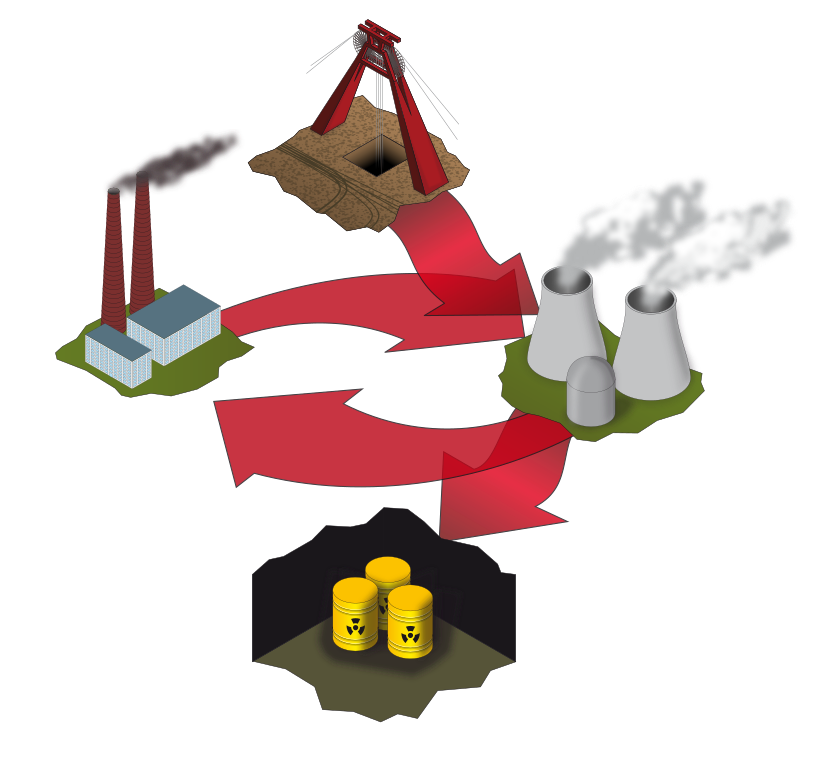
\includegraphics[width=\textwidth]{img/nfc.png}
                \vfill
            \end{tcolorbox}
        \end{minipage}
        \begin{minipage}{.32\linewidth}
            \begin{tcolorbox}[colback=white, colframe=black, width=\linewidth, height=1.55\linewidth, boxrule=1pt]
                \researcharea{Advanced Computation}
                \newline\vfill
                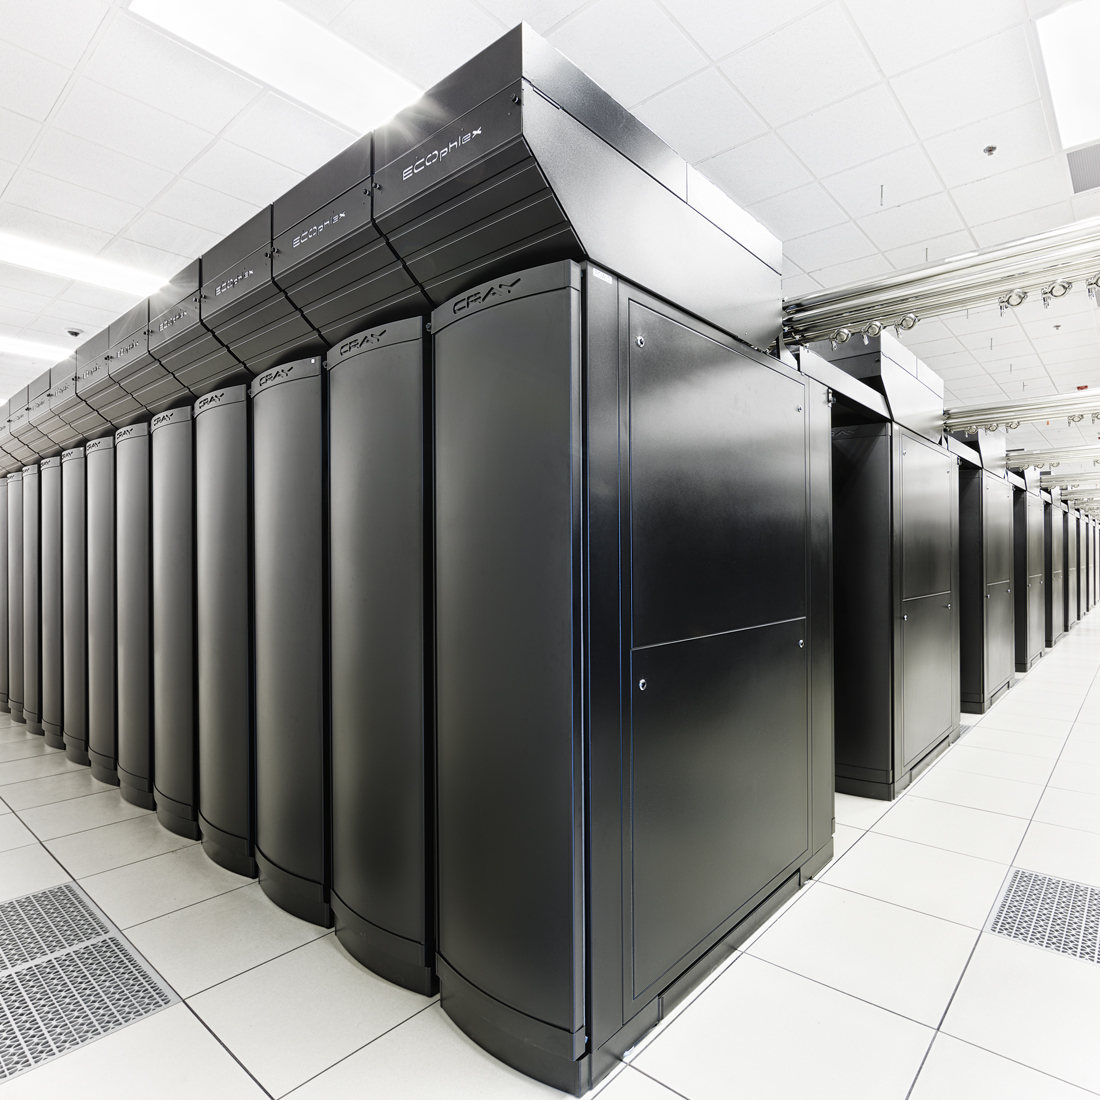
\includegraphics[width=\textwidth]{img/bw_cropped.jpg}
                \vfill
            \end{tcolorbox}
        \end{minipage}
    }

    %%%%%%%%%%%%%%%%%%%%%%%%%
    %%%% Logos of codes %%%%%
    %%%%%%%%%%%%%%%%%%%%%%%%%
    \vspace{-0.5em}
    \begin{tcolorbox}[colback=white, colframe=black, width=0.97\linewidth, height=.32\linewidth, boxrule=1pt]
        \codelogoheader{Open-Source Nuclear Research Codes}
        \sectioncontent{
            \begin{minipage}{.22\linewidth}
                
\includegraphics[width = \linewidth]{img/openmc_logo.png}
                \newline\vspace{0.25em}
                
\includegraphics[width = \linewidth]{img/rollo-logo.png}
            \end{minipage} 
            \begin{minipage}{.22\linewidth}
                
\includegraphics[width =.8\linewidth]{img/pyne.png}
                \vspace{10pt}
            \end{minipage}
            \begin{minipage}{.22\linewidth}
                
\includegraphics[width=.8\linewidth]{img/ghastlylogo.png}
            \end{minipage}
            \begin{minipage}{.22\linewidth}
                
\includegraphics[width=\linewidth]{img/cyclus.png}
                \newline\par\vspace{-0.25em}
                \textcolor{altgeldorange!100}{\textbf{\fontsizemoltres{\texttt{Moltres}}}}\\\vspace{-15pt}
            \end{minipage}
        }
    \end{tcolorbox}

    \vspace{-0.5em}
    %%%%%%%%%%%%%%%%%%%%%%%%%
    %%%%%%%% QR code %%%%%%%%
    %%%%%%%%%%%%%%%%%%%%%%%%%
    \begin{minipage}{.22\linewidth}
        \centering
        
\includegraphics[width=.8\linewidth]{img/qrcode.eps}
        \vspace{-1em}
        \href{https://arfc.github.io/}{\fontsizeauthor\underline{Group Website}}
    \end{minipage}
    %%%%%%%%%%%%%%%%%%%%%%%%%
    %%% Collaborator logos %%
    %%%%%%%%%%%%%%%%%%%%%%%%%
    \begin{minipage}{0.73\linewidth}
        \begin{tcolorbox}[colback=white, colframe=black, width=\linewidth, height=.275\linewidth, boxrule=1pt]
            \begin{center}
                \begin{minipage}{.3\linewidth}
                    \begin{center}
                        %https://www.energy.gov/department-energy-logo-and-branding-guidelines
                        
\includegraphics[width = \linewidth]{img/doe.png}
                        \newline\vspace{-1.5em}
                        %https://www.moltexenergy.com/partners/ornl-logo/
                        
\includegraphics[width = \linewidth]{img/ornl.png}
                    \end{center}
                \end{minipage}
                \begin{minipage}{.3\linewidth}
                    \begin{center}
                        %https://commons.wikimedia.org/wiki/File:NNSA_Logo.png
                        
\includegraphics[width = \linewidth]{img/nnsa.png}
                        \newline\vspace{-1.5em}
                        %https://commons.wikimedia.org/wiki/File:Argonnelablogo.PNG
                        
\includegraphics[width = \linewidth]{img/anl.png}
                    \end{center}
                \end{minipage}
                \begin{minipage}{.3\linewidth}
                    \begin{center}
                        % top left https://en.m.wikipedia.org/wiki/File:US-NuclearRegulatoryCommission-Logo.svg
                        
\includegraphics[width = \linewidth]{img/nrc.png}
                        \newline\par\vspace{-1.5em}
                        % https://inl.gov/logos-videos-images/
                        
\includegraphics[height = .5\linewidth]{img/inl.png}
                    \end{center}
                \end{minipage}
            \end{center}
        \end{tcolorbox}
    \end{minipage}

    %%%%%%%%%%%%%%%%%%%%%%%%%
    %%%%%% References %%%%%%%
    %%%%%%%%%%%%%%%%%%%%%%%%%
    \vspace{-0.5em}
    \begin{tcolorbox}[colback=white, colframe=black, width=1.0\textwidth, arc=6pt, boxrule=1pt]
        \referencestitle{References} % or your preferred title formatting
        \setlength{\columnsep}{0.5em}
        \begin{multicols}{2}
            \fontsizerefs
            \renewcommand{\section}[2]{} % Suppress the automatic section title
            \bibliographystyle{plain}
            \bibliography{group-poster}
        \end{multicols}
    \end{tcolorbox}

    %%%%%%%%%%%%%%%%%%%%%%%%%%%%%
    %%%%%% Logos (UIUC, ARFC) %%%%%%%
    %%%%%%%%%%%%%%%%%%%%%%%%%%%%%%%%%
    
\includegraphics[height=0.28\textwidth]{img/UIUC_Logo.png}\hspace{5cm}
    
\includegraphics[height=0.28\textwidth, trim={0 .5cm 0 .5cm}]{img/arfc_atom.png}
\end{center}
}{
}